\documentclass{article}

\usepackage{graphicx}
\usepackage[hidelinks]{hyperref}
\usepackage{geometry}
\usepackage{amsmath}
\usepackage{listings}
\usepackage{wrapfig}
\usepackage{subcaption}
\usepackage{tikz}
\usetikzlibrary{positioning}

\geometry{
 a4paper,
 left=20mm,
 right=20mm,
 top=20mm,
 bottom=25mm,
}

\begin{document}

\begin{titlepage}
\begin{center}
\vspace*{1cm}
            
\Huge
\textbf{Project 3}
            
\vspace{1cm}

\Large
\text{Due: Tuesday, November 12, 2024}

\vspace{2cm}

\text{\texttt{Brian High}} \\
\text{\texttt{Thomas Hynes}} \\
\text{\texttt{Jeremy Middleman}} \\
\text{\texttt{Andrei Phelps}} \\
\text{\texttt{Wayne Rudnick}} \\

\vspace{2cm}

\includegraphics[scale=0.25]{figs/icon.png}\\[0.5cm]

\vspace{9cm}

\textbf{CS 491/591: Neural Networks} \\

\end{center}
\end{titlepage}
\newpage

\section*{Code Execution}

To run the code, run: \\ \\
Notes: 

\section*{First Section}

\subsection{Newtons Method}

\subsubsection{What is the Hessian?}
The Hessian matrix is a square matrix of second-order partial derivatives. Newton's method's goal is to make a 2nd order approximation and minimize it. The Hessian is how we calculate these 2nd order derivatives. For a function \( F \) with \( n \) parameters, the Hessian is an \( n \times n \) matrix, where each element \( H_{ij} \) represents the second-order partial derivative of \( F \) with respect to two parameters. In our case, the Hessian is \( n \times n \) matrix where n is the number of weights in the neural network. The hessian captures the curvature of the function along each individual parameter axis along with the interaction between pairs of parameters. This structure second-order optimization methods to work. 
\subssection{}
\subsubsection{Resulting Hessians}

\includegraphics[scale=0.1]{../figs/Case 1.png} \\[0.5cm]
\[
H_1 = \begin{bmatrix}
\frac{\partial^2 L}{\partial (w_{1,1}^{[1]})^2} & \frac{\partial^2 L}{\partial w_{1,1}^{[1]} \partial w_{1,1}^{[2]}} & \frac{\partial^2 L}{\partial w_{1,1}^{[1]} \partial w_{1,1}^{[3]}} & \frac{\partial^2 L}{\partial w_{1,1}^{[1]} \partial w_{1,1}^{[4]}} \\
\frac{\partial^2 L}{\partial w_{1,1}^{[2]} \partial w_{1,1}^{[1]}} & \frac{\partial^2 L}{\partial (w_{1,1}^{[2]})^2} & \frac{\partial^2 L}{\partial w_{1,1}^{[2]} \partial w_{1,1}^{[3]}} & \frac{\partial^2 L}{\partial w_{1,1}^{[2]} \partial w_{1,1}^{[4]}} \\
\frac{\partial^2 L}{\partial w_{1,1}^{[3]} \partial w_{1,1}^{[1]}} & \frac{\partial^2 L}{\partial w_{1,1}^{[3]} \partial w_{1,1}^{[2]}} & \frac{\partial^2 L}{\partial (w_{1,1}^{[3]})^2} & \frac{\partial^2 L}{\partial w_{1,1}^{[3]} \partial w_{1,1}^{[4]}} \\
\frac{\partial^2 L}{\partial w_{1,1}^{[4]} \partial w_{1,1}^{[1]}} & \frac{\partial^2 L}{\partial w_{1,1}^{[4]} \partial w_{1,1}^{[2]}} & \frac{\partial^2 L}{\partial w_{1,1}^{[4]} \partial w_{1,1}^{[3]}} & \frac{\partial^2 L}{\partial (w_{1,1}^{[4]})^2}
\end{bmatrix}
\]

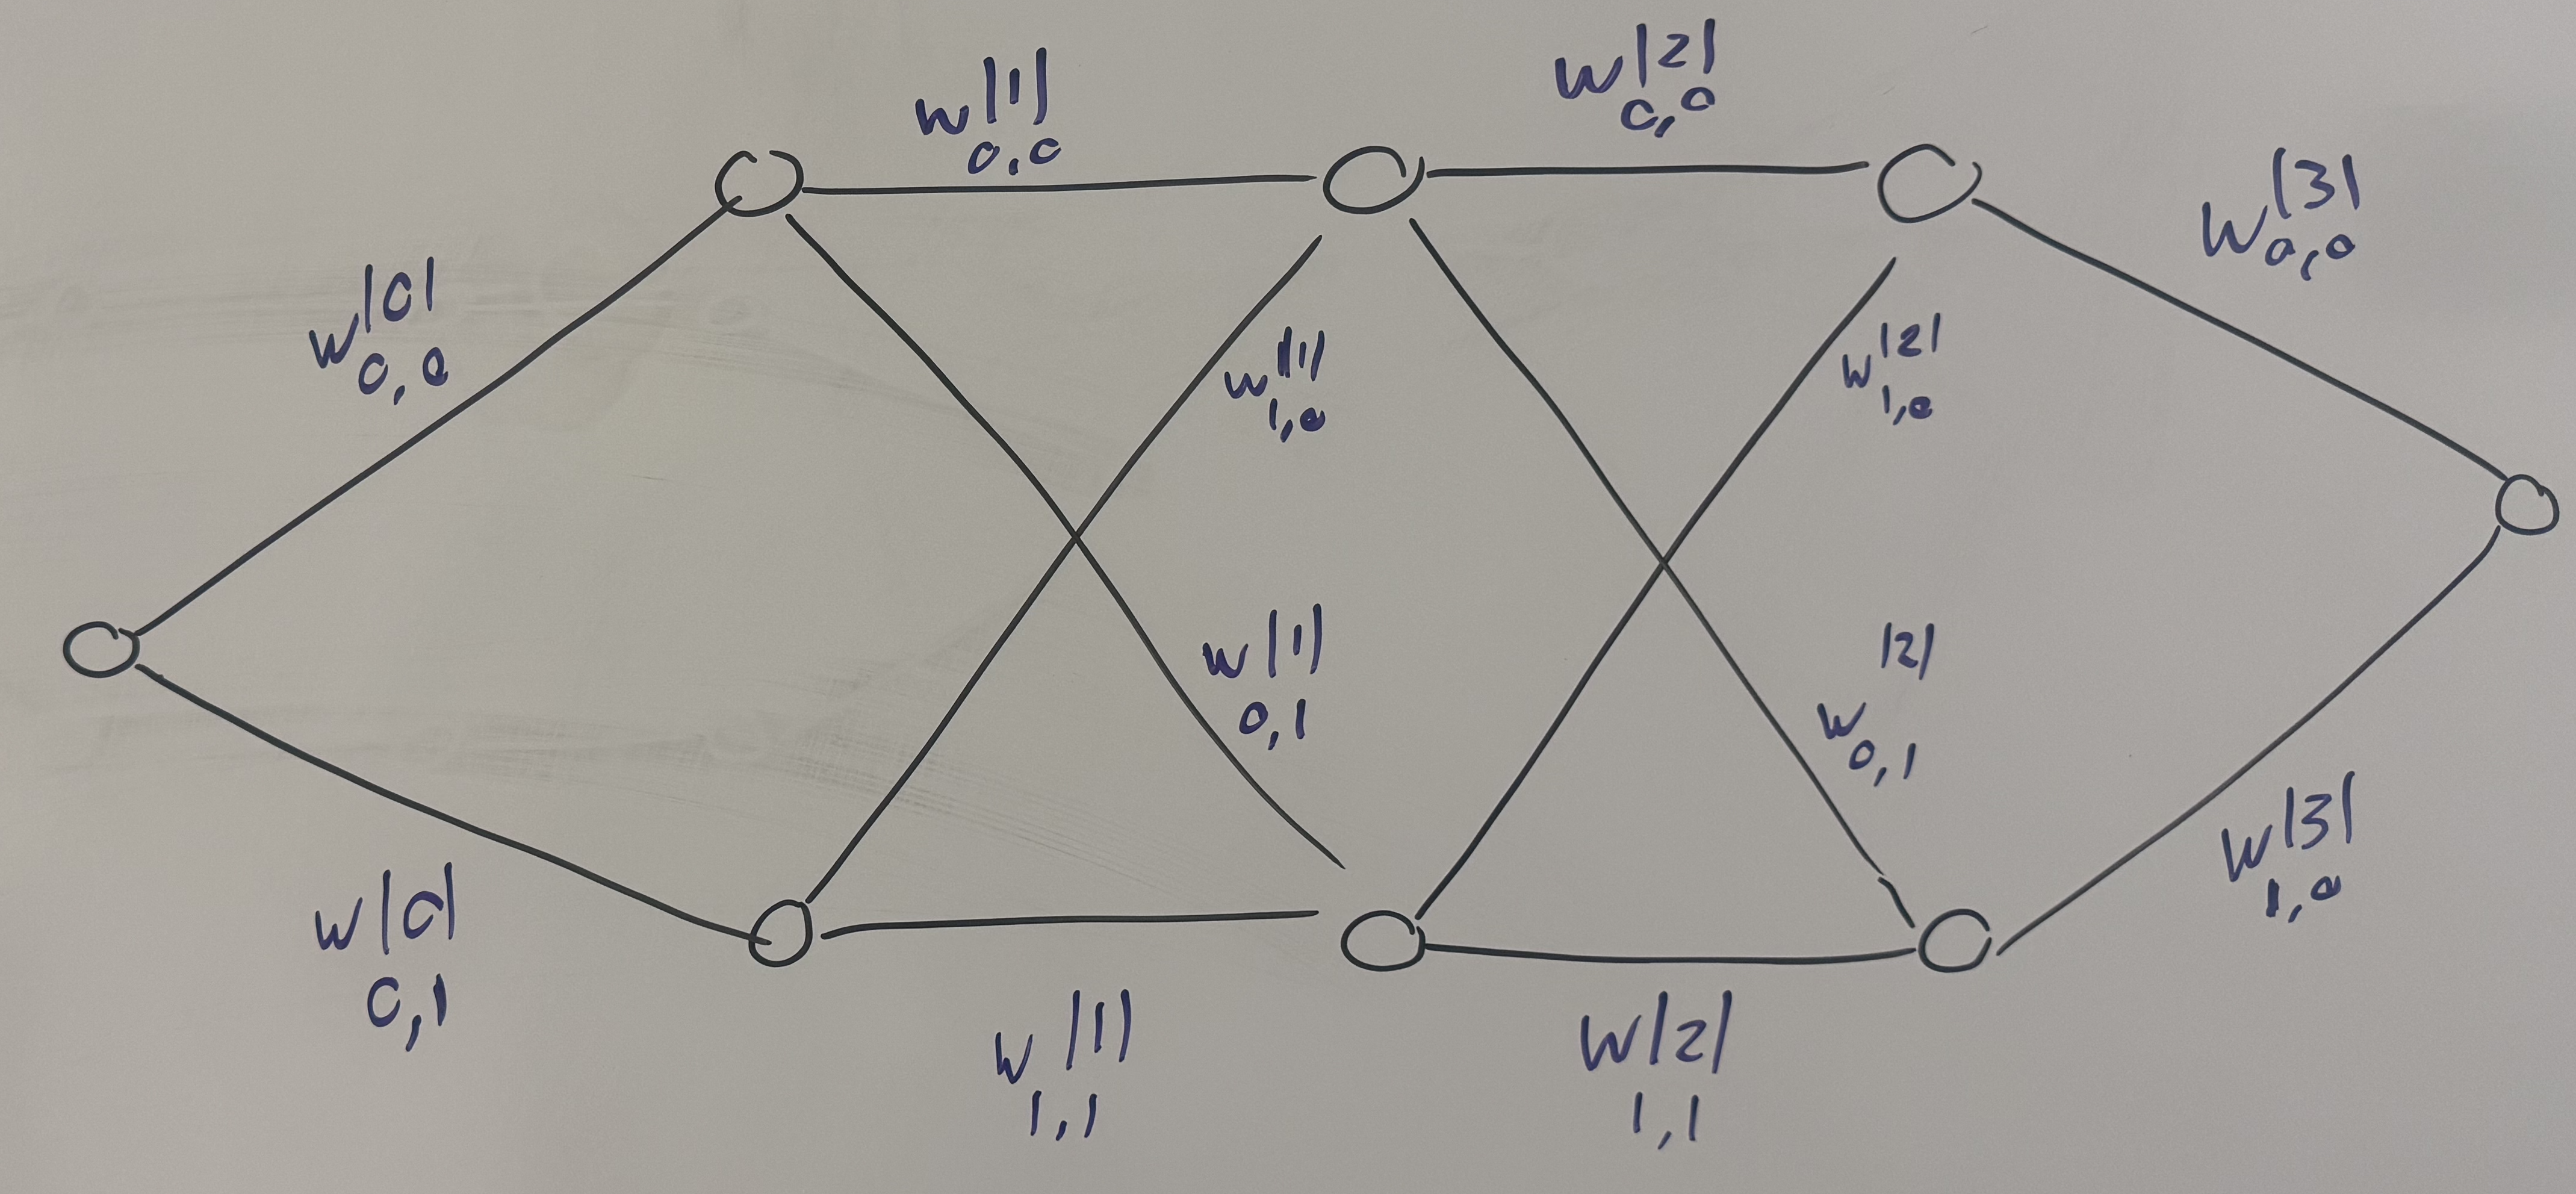
\includegraphics[scale=0.1]{../figs/Case 2.png} \\[0.5cm]

\[
H_2 = \begin{bmatrix}
\frac{\partial^2 L}{\partial (w_{1,1}^{[1]})^2} & \frac{\partial^2 L}{\partial w_{1,1}^{[1]} \partial w_{2,1}^{[1]}} & \cdots & \frac{\partial^2 L}{\partial w_{1,1}^{[1]} \partial w_{2,1}^{[4]}} \\
\frac{\partial^2 L}{\partial w_{2,1}^{[1]} \partial w_{1,1}^{[1]}} & \frac{\partial^2 L}{\partial (w_{2,1}^{[1]})^2} & \cdots & \frac{\partial^2 L}{\partial w_{2,1}^{[1]} \partial w_{2,1}^{[4]}} \\
\vdots & \vdots & \ddots & \vdots \\
\frac{\partial^2 L}{\partial w_{2,1}^{[4]} \partial w_{1,1}^{[1]}} & \frac{\partial^2 L}{\partial w_{2,1}^{[4]} \partial w_{2,1}^{[1]}} & \cdots & \frac{\partial^2 L}{\partial (w_{2,1}^{[4]})^2}
\end{bmatrix}
\]
\section*{Experiments and Results}

\section*{Individual Contributions}

\subsection*{Brian High}
\begin{itemize}
    \item[1)] 
\end{itemize}

\subsection*{Thomas Hynes}
\begin{itemize}
    \item[1)] 
\end{itemize}

\subsection*{Jeremy Middleman}
\begin{itemize}
    \item[1)] 
\end{itemize}

\subsection*{Andrei Phelps}
\begin{itemize}
    \item[1)] 
\end{itemize}

\subsection*{Wayne Rudnick}
\begin{itemize}
    \item[1)] 
\end{itemize}

\end{document}
